

\paragraph{} In this chapter we shall introduce and detail a prototype implementation of a modular, SGX-protected \textit{reference monitor} --- \textsc{Citadel}. First, its necessity will be motivated, and the challenges faced discussed. Then, the three-part architecture will be explained, relating various design decisions to the DIFC model it provides. A discussion about the architecture's performance and effectiveness is provided in §~\ref{sec:eval}.

\section{Motivation}
\paragraph{} Since its introduction in a 1972 report from Anderson~\cite{reference-monitor}, the reference monitor concept has time and again proved to be a reliable workhorse for a plethora of security models. It does not refer to any exact policy, nor limit itself to any particular implementation --- it's abstractness is one of its greatest strengths, reserving any judgement about what policy is \textit{appropriate} in a particular setting.~\cite{irvine-rm}

\paragraph{Fundamental Properties of a Reference Monitor}

\begin{itemize}
    \item \textit{Always invoked.} Every access to the system must be mediated to guarantee that adversaries are unable to bypass the system's security policies.
    \item \textit{Evaluable.} It ``must be small enough to be subject to analysis and tests, the completeness of which can be assured'';~\cite{reference-monitor} to be trustworthy, it must be \textit{auditable}, with, ideally, a restricted TCB.
    \item \textit{Tamper proof.} To ensure that an attacker cannot disable the access control and authorisation steps mandated by the security policy, the integrity of a reference monitor cannot be in question.
\end{itemize}

\paragraph{} No computer system is every completely secure, and Linux is no exception. Having grown by a 1.7 million lines of code (LoC) in the past year alone, now standing at 27.8 million LoC in total,\footnote{\url{https://www.theregister.com/2020/01/06/linux\_2020\_kernel\_systemd\_code/}} bugs are inevitable --- almost 2000 have been reported in the past year,\footnote{\url{https://bugzilla.kernel.org/}} and 662 \textit{severe} bugs are still outstanding.\footnote{\url{https://www.cvedetails.com/product/47/Linux-Linux-Kernel.html}} In this context we must question whether Linux alone can provide a reference monitor implementation the guarantees it requires,~\cite{Lipp2018MeltdownRK, 10.5555/2831143.2831164} thus motivating the use of SGX.

\paragraph{} Applying SGX to this problem brings two attactive benefits;
\begin{itemize}
    \item The system's IFC policy can be evaluable both during offline analysis and online using \textit{attestation}, helping other enclaves' confidence in the underlying system.
    \item SGX's hardware protections are very capable at defending a reference monitor's state, even if adversaries have ring-0 privilege or in the presence of a kernel bug.
\end{itemize}

\section{Challenges}



\clearpage
\begin{figure}[]
    \centering
    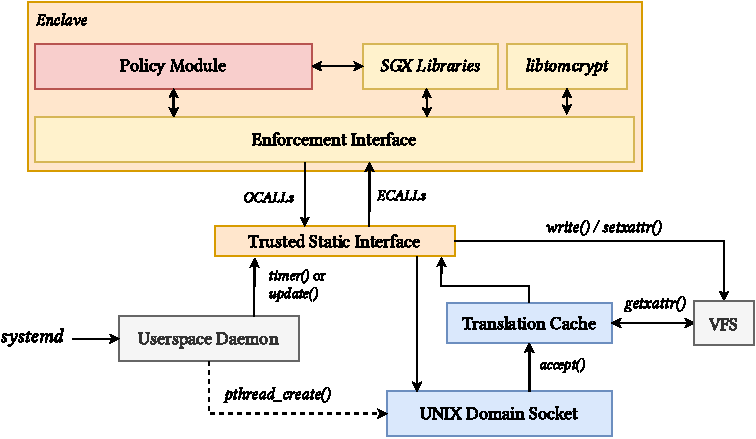
\includegraphics[width=\linewidth]{figures/EnclaveLayout.pdf}
    \caption{Abstract overview of an SGX enclave's protections.}
    \label{fig:sgx-basic}
\end{figure}